\section{Experimental Results}
\subsection{In-Domain Classification Results}
Table~\ref{tab:nick} compares the four-class test results. ResNet-50 has the highest mean accuracy, 99.14\%, but requires 23.52M parameters, 8.17 GFLOPs, and 67.89 ms per image. LS-Net obtains 98.29\% accuracy with 0.91M parameters, 0.36 GFLOPs, and 11.30 ms. Thus its mean accuracy is 0.85 percentage points lower while its measured CPU latency is about six times smaller. We treat this as an accuracy--latency trade-off; LS-Net remains below the larger model in absolute accuracy. EfficientNet-Tiny uses fewer FLOPs but has higher reported latency than LS-Net; neither the smallest parameter count nor the lowest operation count alone identifies the fastest model.

\begin{table*}[t]
\caption{In-Domain Performance and Edge Efficiency on Nickparvar Four-Class MRI}\label{tab:nick}
\centering\scriptsize
\resizebox{\textwidth}{!}{\begin{tabular}{llrrrrrrrr}
\toprule
Architecture & Training & Params (M) & GFLOPs & Latency (ms) & FPS & Accuracy (\%) & Macro F1 (\%) & Specificity (\%) & AUC (\%) \\
\midrule
\textbf{ResNet-50} & Fine-tuned & 23.52 & 8.17 & 67.89 & 14.7 & $\mathbf{99.14\pm0.16}$ & $\mathbf{99.15\pm0.17}$ & $99.71\pm0.06$ & $99.92\pm0.05$ \\
EfficientNet-B0 & Fine-tuned & 4.01 & 0.77 & 23.91 & 41.8 & $99.08\pm0.28$ & $99.08\pm0.27$ & $99.70\pm0.09$ & $\mathbf{99.97\pm0.02}$ \\
VGG-16 & Fine-tuned & 27.56 & 30.72 & 150.03 & 6.7 & $98.86\pm0.10$ & $98.86\pm0.10$ & $99.62\pm0.03$ & $99.94\pm0.03$ \\
ResNet-18 & Fine-tuned & 11.18 & 3.63 & 27.96 & 35.8 & $98.70\pm0.47$ & $98.70\pm0.47$ & $99.57\pm0.16$ & $99.94\pm0.02$ \\
MobileNetV2 & Fine-tuned & 2.23 & 0.60 & 17.35 & 57.6 & $98.45\pm0.33$ & $98.45\pm0.33$ & $99.48\pm0.11$ & $99.95\pm0.03$ \\
\midrule
\textbf{LS-Net} & Scratch & \textbf{0.91} & \textbf{0.36} & \textbf{11.30} & \textbf{88.5} & $\mathbf{98.29\pm0.25}$ & $\mathbf{98.29\pm0.25}$ & $99.43\pm0.08$ & $99.79\pm0.08$ \\
MPAC-ResNet-Tiny & Scratch & 0.72 & 0.92 & 18.01 & 55.5 & $98.22\pm0.30$ & $98.22\pm0.30$ & $99.41\pm0.11$ & $99.84\pm0.03$ \\
EfficientNet-Tiny & Scratch & 0.75 & 0.19 & 16.14 & 61.9 & $98.13\pm0.38$ & $98.14\pm0.38$ & $99.38\pm0.13$ & $99.85\pm0.04$ \\
MPAC-ResNet & Fine-tuned & 1.86 & 2.17 & 19.50 & 51.3 & $98.10\pm0.44$ & $98.10\pm0.44$ & $99.37\pm0.14$ & $99.82\pm0.05$ \\
ResNet-Tiny & Scratch & 0.98 & 2.51 & 24.19 & 41.3 & $97.72\pm0.17$ & $97.72\pm0.16$ & $99.24\pm0.05$ & $99.78\pm0.03$ \\
MobileNet-Tiny & Scratch & 0.40 & 0.12 & 11.43 & 87.5 & $97.65\pm0.14$ & $97.67\pm0.14$ & $99.22\pm0.05$ & $99.78\pm0.04$ \\
\bottomrule
\end{tabular}}
\end{table*}

\begin{figure*}[t]
\centering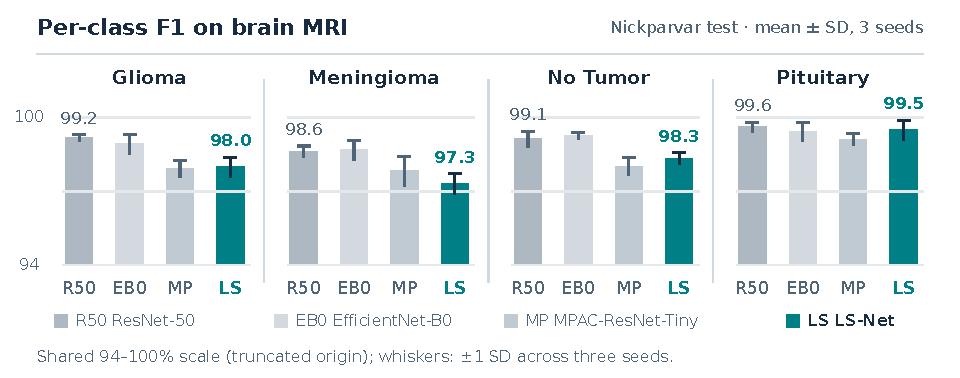
\includegraphics[width=0.82\textwidth]{figures/model_class_comparison.pdf}
\caption{Nickparvar per-class F1 (three-seed mean, whiskers $\pm1$ SD). R50/EB0: fine-tuned ResNet-50/EfficientNet-B0; LS/MP: scratch-trained LS-Net/MPAC-ResNet-Tiny. LS-Net is highlighted. All bars share a truncated 94--100\% axis.}\label{fig:model-class-compare}
\end{figure*}

To examine whether a small numerical accuracy difference is consistently reflected in paired test errors, Table~\ref{tab:stats} gives seed-specific McNemar $p$-values. ResNet-50 versus LS-Net yields $0.109$, $0.078$, and $0.125$: none passes the nominal significance threshold. This does not establish that the models are clinically interchangeable or statistically equivalent; it indicates that the paired test does not detect a difference on these held-out predictions. Class-level F1 adds important context (Table~\ref{tab:classes} and Fig.~\ref{fig:model-class-compare}): LS-Net records 97.32\% on meningioma, its lowest among the four categories, versus 99.50\% on pituitary. Aggregate accuracy alone therefore understates differences among tumor categories.

\begin{table*}[t]
\caption{Per-Class F1-Score Breakdown on Nickparvar Four-Class (\%)}\label{tab:classes}
\centering\scriptsize
\resizebox{\textwidth}{!}{\begin{tabular}{lrrrr}
\toprule
Model & Glioma F1 (\%) & Meningioma F1 (\%) & No Tumor F1 (\%) & Pituitary F1 (\%) \\
\midrule
ResNet-50 & $99.19\pm0.11$ & $98.63\pm0.22$ & $99.14\pm0.30$ & $99.62\pm0.19$ \\
EfficientNet-B0 & $98.94\pm0.39$ & $98.69\pm0.38$ & $99.27\pm0.12$ & $99.43\pm0.38$ \\
VGG-16 & $98.87\pm0.19$ & $98.39\pm0.21$ & $98.81\pm0.20$ & $99.37\pm0.39$ \\
ResNet-18 & $98.69\pm0.49$ & $97.94\pm0.65$ & $98.81\pm0.53$ & $99.37\pm0.29$ \\
\midrule
\textbf{LS-Net} & $\mathbf{98.00\pm0.39}$ & $\mathbf{97.32\pm0.40}$ & $\mathbf{98.35\pm0.22}$ & $\mathbf{99.50\pm0.39}$ \\
MPAC-ResNet-Tiny & $97.93\pm0.33$ & $97.83\pm0.59$ & $98.02\pm0.35$ & $99.12\pm0.22$ \\
\textbf{MCG-TTA (proposed)} & $\mathbf{98.15\pm0.18}$ & $\mathbf{97.60\pm0.22}$ & $\mathbf{98.42\pm0.19}$ & $\mathbf{99.52\pm0.09}$ \\
\bottomrule
\end{tabular}}
\end{table*}

Fig.~\ref{fig:mri-examples} contrasts a correct glioma classification with a false-positive no-tumor slice. The attribution maps are not validated lesion localization.

\begin{figure*}[t]
\centering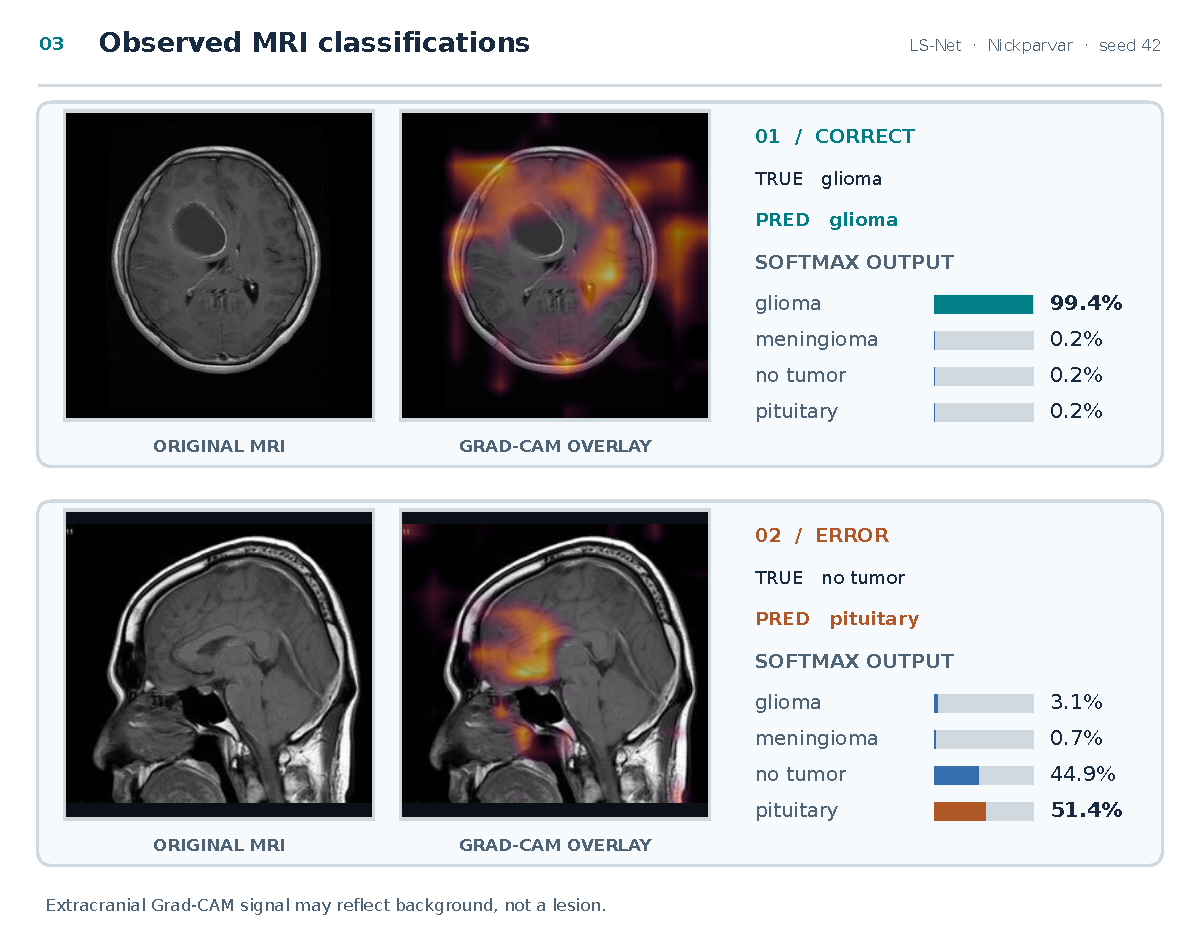
\includegraphics[width=0.85\textwidth]{figures/mri_classification_examples.pdf}
\caption{Held-out Nickparvar slices (LS-Net, seed 42). Left: correctly classified glioma. Right: false-positive no-tumor slice predicted as pituitary (confidence $\approx50\%$). Grad-CAM overlays use the third MPAC stage; they indicate class-discriminative regions without validating lesion boundaries.}\label{fig:mri-examples}
\end{figure*}

\begin{table*}[t]
\caption{Pairwise McNemar Statistical Tests on Test Set ($N=1{,}052$)}\label{tab:stats}
\centering\scriptsize
\begin{tabular}{lrrrl}
\toprule
Comparison & Seed 42 ($p$-value) & Seed 123 ($p$-value) & Seed 456 ($p$-value) & Statistical Decision ($\alpha=0.05$) \\
\midrule
ResNet-50 vs. EfficientNet-B0 & $p=1.000$ & $p=0.625$ & $p=0.500$ & Not significant \\
ResNet-50 vs. LS-Net & $p=0.109$ & $p=0.078$ & $p=0.125$ & Not significant \\
LS-Net vs. MPAC-ResNet-Tiny & $p=0.727$ & $p=0.815$ & $p=1.000$ & Not significant \\
MPAC-Tiny vs. EfficientNet-Tiny & $p=0.480$ & $p=0.804$ & $p=1.000$ & Not significant \\
\bottomrule
\end{tabular}
\end{table*}

\subsection{Cross-Dataset Glioma Grading}
The advantage of a balanced and nearly saturated benchmark is that it reveals the cost of shrinking a model under favorable conditions; its limitation is that it cannot demonstrate robustness in a distinct task. Table~\ref{tab:brats} reports the separately trained BraTS 2020 HGG/LGG results. Here VGG-16 leads at 89.31\% slice macro F1, whereas LS-Net reaches 82.02\% and ResNet-Tiny 84.57\%. Architecture rankings also change: MobileNet-Tiny falls to 68.89\% slice F1, despite its 97.67\% macro F1 on the four-class benchmark. The numbers compare performance across two separately trained tasks; no four-class weights were applied to grading. Their difference cannot be attributed solely to dataset shift because labels, class frequencies, and training data differ as well.

\begin{table*}[t]
\caption{Cross-Dataset Generalization and Clinical Grading on BraTS 2020}\label{tab:brats}
\centering\scriptsize
\resizebox{\textwidth}{!}{\begin{tabular}{lrrrrrrr}
\toprule
Model & Params (M) & Slice F1 (\%) & Slice Acc. (\%) & Slice AUC (\%) & Patient F1 (\%) & Patient Acc. (\%) & LGG Recall (/ 12) \\
\midrule
\textbf{VGG-16} & 27.56 & $\mathbf{89.31\pm0.06}$ & $\mathbf{92.57\pm0.10}$ & $\mathbf{96.25\pm0.93}$ & $\mathbf{92.34\pm3.33}$ & \textbf{94.64} & \textbf{11.0 / 12} \\
ResNet-50 & 23.52 & $84.76\pm0.86$ & $89.65\pm1.21$ & $94.85\pm0.54$ & $87.91\pm1.10$ & 91.96 & 9.5 / 12 \\
ResNet-Tiny & 0.98 & $84.57\pm2.92$ & $90.07\pm1.92$ & $94.71\pm1.14$ & $84.68\pm2.33$ & 90.18 & 8.5 / 12 \\
EfficientNet-B0 & 4.01 & $84.46\pm0.99$ & $88.90\pm0.15$ & $94.82\pm1.01$ & $90.04\pm3.17$ & 92.86 & \textbf{11.0 / 12} \\
\midrule
\textbf{MCG-TTA (proposed)} & \textbf{0.91} & $\mathbf{83.45\pm2.07}$ & $\mathbf{88.83\pm1.04}$ & $90.74\pm3.20$ & $\mathbf{88.15\pm1.83}$ & 91.97 & 10.0 / 12 \\
MPAC-ResNet & 1.86 & $82.26\pm2.28$ & $86.93\pm3.03$ & $93.14\pm0.23$ & $83.90\pm0.27$ & 88.39 & 10.0 / 12 \\
LS-Net (base) & \textbf{0.91} & $82.02\pm2.36$ & $88.25\pm0.86$ & $89.82\pm4.29$ & $\mathbf{89.33\pm0.92}$ & 92.86 & 10.0 / 12 \\
ResNet-18 & 11.18 & $81.08\pm1.05$ & $85.75\pm0.16$ & $93.46\pm1.04$ & $80.88\pm1.29$ & 85.71 & 10.0 / 12 \\
MPAC-ResNet-Tiny & 0.72 & $80.06\pm3.07$ & $86.93\pm2.93$ & $91.26\pm3.53$ & $83.56\pm0.75$ & 89.29 & 8.5 / 12 \\
MobileNetV2 & 2.23 & $78.87\pm1.15$ & $85.32\pm0.76$ & $91.21\pm0.46$ & $79.40\pm3.64$ & 85.71 & 8.5 / 12 \\
EfficientNet-Tiny & 0.75 & $76.00\pm1.03$ & $80.78\pm0.60$ & $89.09\pm0.49$ & $80.38\pm5.67$ & 83.93 & \textbf{11.5 / 12} \\
MobileNet-Tiny & 0.40 & $68.89\pm5.36$ & $74.68\pm5.50$ & $82.57\pm6.44$ & $71.09\pm4.69$ & 76.79 & 9.0 / 12 \\
\bottomrule
\end{tabular}}
\end{table*}

Slice and patient rankings are not identical. For example, baseline LS-Net has 89.33\% patient F1 in Table~\ref{tab:brats} despite 82.02\% slice F1. This is consistent with averaging many slice probabilities into one patient decision, but no claim of independent per-slice evidence follows: slices within a patient are correlated. In particular, high aggregate accuracy under an HGG-heavy test set should be checked against LGG recall. The reported mean of 10.0/12 LGG cases detected per seed for LS-Net corresponds to a substantive residual miss rate.

\begin{figure*}[t]
\centering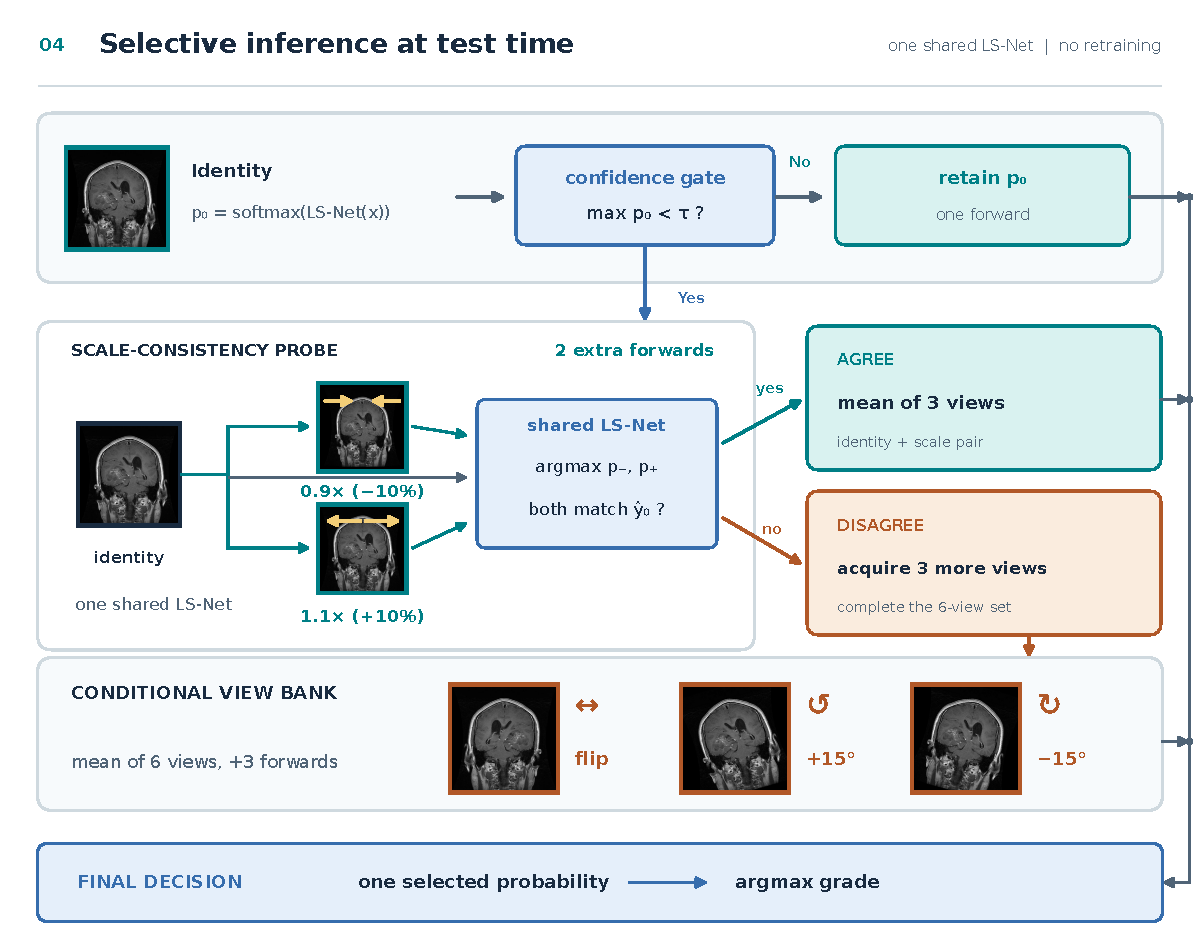
\includegraphics[width=0.85\textwidth]{figures/mcg_tta.pdf}
\caption{MCG-TTA inference rule for the BraTS grading task. A confident prediction exits after one forward pass. A gated slice receives two scale probes; agreement averages three probability vectors, whereas disagreement adds a flip and two rotations before averaging all six.}\label{fig:mcg-tta}
\end{figure*}

\subsection{Ablation Study}
Table~\ref{tab:tta} isolates the inference strategy on BraTS. MCG-TTA changes neither the LS-Net weights nor its 0.91M parameters, increasing mean slice F1 from 82.02\% to 83.45\%. In seed 42 the gain is 85.52\% minus 83.69\%, or 1.83 percentage points; across the two tabulated seeds the gain is 1.43 points. The 27.6\% confidence-trigger rate and 3.3 additional forwards per triggered slice yield a modelled 10.74 ms per slice versus 5.60 ms for the baseline, a 1.92$\times$ ratio. The cost is not six full views for all cases: non-triggered slices remain single-pass.

\begin{table*}[t]
\caption{Ablation of Test-Time Augmentation Strategies on LS-Net (BraTS 2020)}\label{tab:tta}
\centering\scriptsize
\resizebox{\textwidth}{!}{\begin{tabular}{llrrrrlrrr}
\toprule
Strategy & Gating / Probe Rule & Trigger (\%) & Extra/Trig. & Modelled (ms) & Rel. Cost & Slice F1 (s42/s123) & Mean F1 (\%) & Patient F1 (\%) & LGG Recall (/ 24) \\
\midrule
LS-Net (Base) & Single standard forward pass & 0.0 & 0 & \textbf{5.60} & \textbf{1.00$\times$} & 83.69 / 80.35 & 82.02 & \textbf{89.34} & \textbf{20 / 24} \\
\texttt{disagree} & $p_{\max} < \tau \to$ flip probe; escalate on argmax change & 27.6 & 2.0 & 8.73 & 1.56$\times$ & 85.84 / 81.22 & 83.53 & 86.24 & 18 / 24 \\
\textbf{MCG-TTA (proposed)} & \textbf{$p_{\max} < \tau \to$ scale $\pm10\%$ probes; escalate on disagreement} & \textbf{27.6} & \textbf{3.3} & \textbf{10.74} & \textbf{1.92$\times$} & \textbf{85.52 / 81.38} & \textbf{83.45} & \textbf{88.15} & \textbf{20 / 24} \\
\texttt{conf} & $p_{\max} < \tau \to$ execute all 6 augmentations & 27.6 & 5.0 & 13.28 & 2.37$\times$ & 85.35 / 81.34 & 83.35 & 88.15 & \textbf{20 / 24} \\
\texttt{weakclass} & Trigger on $p_{\max} < \tau$ OR predicted LGG & 39.7 & 5.0 & 16.65 & 2.97$\times$ & 85.23 / 80.93 & 83.08 & 85.08 & 18 / 24 \\
\texttt{subject} & Escalate all slices of low-confidence patients & 100 (pat.) & 5.0 & 13.82 & 2.47$\times$ & 84.31 / 80.67 & 82.49 & 84.00 & 18 / 24 \\
\midrule
Full TTA (Ceiling) & Unconditional 6-view TTA on all samples & 100.0 & 5.0 & 33.60 & 6.00$\times$ & 85.44 / -- & -- & 87.13 & 19 / 24 \\
\bottomrule
\end{tabular}}
\end{table*}

The full six-view cost of 33.60 ms is the modelled $6\times5.60$-ms forward-pass cost, not a directly timed adaptive pipeline. The flip-disagreement gate has a marginally higher mean slice F1 (83.53\%) than MCG-TTA (83.45\%) at lower modelled latency, but it reduces patient F1 to 86.24\% and LGG detections from 20/24 to 18/24. The proposed rule is consequently not the top method by slice F1 alone; its distinction is the observed combination of slice-level recovery, a smaller compute burden than confidence-only full views, and no additional LGG misses relative to the baseline in the two-seed ablation. It \emph{preserves the baseline's 20 detections out of 24 pooled LGG cases}. Patient F1 nevertheless decreases from the baseline's approximately 89.34\% to 88.15\%; the clinical trade-off should not be hidden behind the slice-level gain. Unconditional six-view TTA has no mean slice F1 because it was evaluated on only one seed.

\subsection{Deployment Cost Analysis}
Table~\ref{tab:edge} records the hardware-facing profile separately from the TTA ablation. LS-Net needs 3.49 MB of model storage, whereas ResNet-50 needs 89.71 MB. Combining the 1.92$\times$ TTA relative cost with the independent 11.30-ms LS-Net CPU timing gives an \emph{estimated} 21.47-ms effective latency and 46.6 FPS; these values are extrapolations. Even under that estimate, the adaptive system remains smaller in storage and faster in modelled inference than the 67.89-ms ResNet-50 baseline. End-to-end preprocessing, image loading, and deployment on actual clinical equipment remain unmeasured.

\begin{table*}[t]
\caption{Edge Hardware Profiling and Computational Complexity}\label{tab:edge}
\centering\scriptsize
\resizebox{\textwidth}{!}{\begin{tabular}{llrrrrrrr}
\toprule
Category & Architecture & Params (M) & Size (MB) & GFLOPs & GMACs & Latency (ms) & FPS & Speedup vs. R50 \\
\midrule
\textit{Heavyweight Baselines} & VGG-16 & 27.56 & 105.14 & 30.72 & 15.36 & 150.03 & 6.7 & $0.45\times$ \\
& ResNet-50 & 23.52 & 89.71 & 8.17 & 4.09 & 67.89 & 14.7 & $1.00\times$ (Ref) \\
& ResNet-18 & 11.18 & 42.64 & 3.63 & 1.81 & 27.96 & 35.8 & $2.43\times$ \\
& EfficientNet-B0 & 4.01 & 15.31 & 0.77 & 0.39 & 23.91 & 41.8 & $2.84\times$ \\
& MobileNetV2 & 2.23 & 8.50 & 0.60 & 0.30 & 17.35 & 57.6 & $3.91\times$ \\
\midrule
\textit{Compact Models ($<2$M)} & MPAC-ResNet & 1.86 & 7.10 & 2.17 & 1.08 & 19.50 & 51.3 & $3.48\times$ \\
& ResNet-Tiny & 0.98 & 3.72 & 2.51 & 1.26 & 24.19 & 41.3 & $2.81\times$ \\
& \textbf{LS-Net (base)} & \textbf{0.91} & \textbf{3.49} & \textbf{0.36} & \textbf{0.18} & \textbf{11.30} & \textbf{88.5} & \textbf{6.01$\times$} \\
& \textbf{MCG-TTA (proposed)} & \textbf{0.91} & \textbf{3.49} & $\sim0.68$ & $\sim0.34$ & $\sim21.47$ & $\sim46.6$ & $\sim3.16\times$ \\
& EfficientNet-Tiny & 0.75 & 2.88 & 0.19 & 0.09 & 16.14 & 61.9 & $4.21\times$ \\
& MPAC-ResNet-Tiny & 0.72 & 2.74 & 0.92 & 0.46 & 18.01 & 55.5 & $3.77\times$ \\
& MobileNet-Tiny & 0.40 & 1.53 & 0.12 & 0.06 & 11.43 & 87.5 & $5.94\times$ \\
\bottomrule
\end{tabular}}
\end{table*}
